\documentclass[12pt,titlepage]{article}





%PACKAGES
\usepackage[ngerman]{babel}
\usepackage[utf8]{inputenc}
\usepackage[a4paper,lmargin={2.5cm},rmargin={2.5cm},
tmargin={2.5cm},bmargin = {2.5cm}]{geometry}
\usepackage{graphicx}
\usepackage{caption}
\usepackage{float}
\usepackage{hyperref}
\parindent0pt





\begin{document}



\thispagestyle{empty}

%TITELSEITE
\begin{center}
\textbf{Hochschule Luzern}\\
Departement für Informatik\\[12\baselineskip]

\begin{Huge}
Projekt FoodPrint
\end{Huge} \\[6\baselineskip]

\begin{large}
\textbf{Programmieren fürs IOS}
\end{large} \\[6\baselineskip]

\begin{large}
\textbf{Studierende}: Frederico Fischer, Nico Iseli\\
\textbf{Dozenten}: Prof. Dr. Ruedi Arnold, Nicolas Märki\

\textbf{Abgabedatum}: 13. Dezember 2020 \\ 
\end{large}
\end{center}
\newpage


\section*{Einleitung}
Das vorliegende Projekt hat zum Ziel, eine App zu entwickeln, die Leute mehr zu unweltfreundlichen Einkäufen ermutigt. Die App soll dabei bedürfnisbasiert regionale und saisonale Produkte vorschlagen. Die Implementierung ist vorerst für User aus der Schweiz vorgesehen. Das Datenbankschema im Backend ist jedoch so aufgebaut, dass sich das App auch auf weitere Länder skalieren lässt.

\section*{Architektur}
Die Architektur ist so aufgebaut, dass Produktdaten im JSON-Format über einen Webserver, der durch das EnterpriseLab gehostet wird, zur Verfügung gestellt werden. Die Produktdaten werden über HTTP-Requests geladen und mittels Core-Data persistiert. Beim Laden wird jeweils geprüft, ob es auf dem Server Änderung der Produktdaten gab. Falls nein, werden die Produktdaten im App auch nicht angepasst. Neben den Produktdaten werden auch die User-Einstellungen mittels Core-Data festgehalten. Die User-Daten befinden sich jedoch nur App-Intern. Die User-Daten werden genutzt, um die Produkte user-spezifisch zu filtern. Für das User-Interface setzt das Projektteam auf UI-Kit.Die Architektur ist ebenfalls als Abbildung (vgl. Abbildung \ref{img: Architektur} auf Seite \pageref{img: Architektur}) festgehalten.\\
\begin{figure}[H]
	\centering
	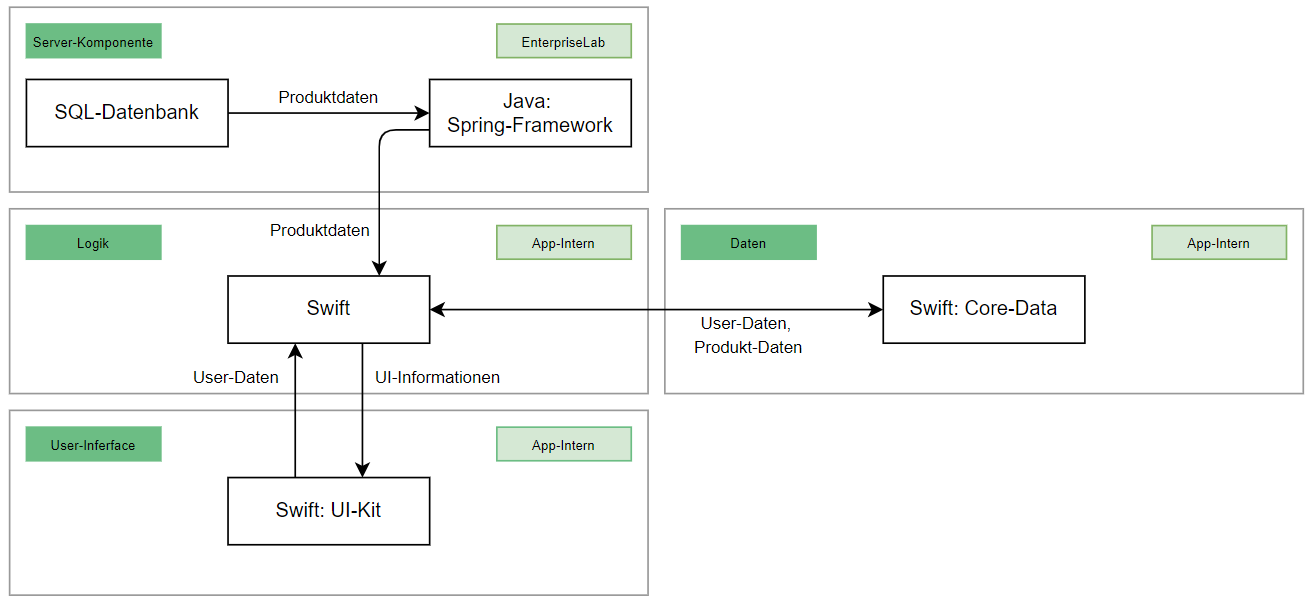
\includegraphics[width=16cm]{Img/Architektur.png}
	\caption[Architektur]{Architektur,\\ Quelle: Projektteam}
	\label{img: Architektur}
\end{figure}

\section*{Server-Komponente}
Für die Server-Komponente wurde eine Ressource im EnterpriseLab reserviert. Dort werden die Produktdaten in einer SQL-Datenbank festgehalten und mit Java (beziehungsweise dessen Framework Sprint) verarbeitet. Die Produktdaten werden auf dem Server in ein JSON-Format konvertiert und über den Webserver zur Verfügung gestellt (ersichtlich unter: \url{http://ffischer-ios-h20.el.eee.intern:8080/api/v1/products/Schweiz}). Aktuell läuft der Server nicht in der DMZ. Daher ist ein Aufruf nur mit bestehender VPN-Verbindung möglich.\\
\\
\textbf{Code-Referenz: }\path{foodprint-backend-distribution}

\section*{HTTP-Kommunikation}
Die JSON-Daten des Webservers werden über den Aufruf der  URL geladen und mittels des JSON-Decoders von Swift in ein Array von Swift-Objekten konvertiert.\\
\\
\textbf{Code-Referenz: }\\ \path{IOS_App_Project/FoodPrint/ FoodPrint/ViewControllers/ProductListViewController.swift/(MARK: - API)}

\section*{Persistierung mit Core-Data}
Mittels Core-Data werden die User-Daten sowie die Produktdaten lokal persistiert. Die App verwaltet dabei ingesamt einen User und mehrere Produktdaten. Diese können gelesen (über die Fetch-Methode im NSManagedContext) und persistiert (über die Save-Methode im NSManagedContext) werden. Der persistierte User dient dazu, die eigenen Bedürfnisse zu ändern und demzufolge die entsprechenden Produktdaten zu filtern.\\
\\
\textbf{Code-Referenz: }\\ \path{IOS_App_Project / FoodPrint / FoodPrint / Utils / CoreData.swift}


\section*{Verwendung von Nebenläufigkeit}
Nebenläufigkeit kam ausschliesslich beim Holen der Daten über die API zum Einsatz. Falls die Produktdaten aktualisiert werden müssen, werden diese beim Start der App Nebenläufig abgerufen.\\
\\
\textbf{Code-Referenz: }\\ \path{IOS_App_Project / FoodPrint / FoodPrint / ViewControllers / ProductListViewController.swift / (MARK: - API)}


\section*{Unit-Tests}
Text\\
\\
\textbf{Code-Referenz: }\\ \path{IOS_App_Project / FoodPrint / FoodPrintTests / FoodPrintTests.swift}

\section*{Auto-Layout}
Für das Projekt wurden die verschiedenen Inhalte der einzelnen View-Controller mittels Auto-Layout formatiert. Dafür wurden entsprechende Contraints gesetzt. Die Nutzung dieses Features wurde jedoch zu wenig gut geplant. Dieses wurde ohne grosses Vorwissen genutzt, was dazu führte, dass die Contraints mehrmals gelöscht und wieder neu erstellt werden mussten. Zudem wurden auch zu wenig Geräte getestet. Aktuell sieht die Formatierung auf neueren beziehungsweise grösseren Geräten gut aus. Hingegen auf kleineren Geräten (beispielsweise auf dem I Phone SE) überlappen sich einige Inhalte. Um dies zu beheben, wurde versucht, im Nachhinein noch eine Scroll-View zu integrieren. Diese kam dann jedoch mit den bestehenden Contraints in Konflikt. Daher ist die App aktuell nicht auf alle Geräte ausgelegt.\\
\\
\textbf{Code-Referenz: }\\ \path{IOS_App_Project / FoodPrint / FoodPrint / Utils / Main.storyboard}

\section*{Erkenntnisse}
Das Erstellen einer eigenen App war eine sehr interessante Erfahrung. Das Wissen über das IOS sowie Swift hat sich im Team durch das Projekt sicherlich verbessert. Insgesamt wurden einige Fehler gemacht, ohne die man im Nachhinein sicherlich effizienter gewesen wäre. Ein Beispiel dafür ist die Nutzung von Auto-Layout. Ein Problem dabei war es, dass zu schnell damit begonnen wurde. Es mussten immer wieder Constraints gelöscht und neu erstellt werden. Ein anderes Beispiel ist das Datenmanagement. Hier wurden die bisherigen Produktdaten von Hand abgetragen, weil keine passende Referenz gefunden wurde. Kämen neue Produkte dazu, müsste die Datenerhebung überdacht werden. Abgesehen davon ist man aber mit dem Resultat sehr zufrieden und motviert, die App auch im Anschluss an die Projektabgabe weiterzuführen.










\end{document}